\chapter{Aufgabe 11}
\section{Aufgabe 11.1}

\begin{wrapfigure}[21]{r}{.4\textwidth}
	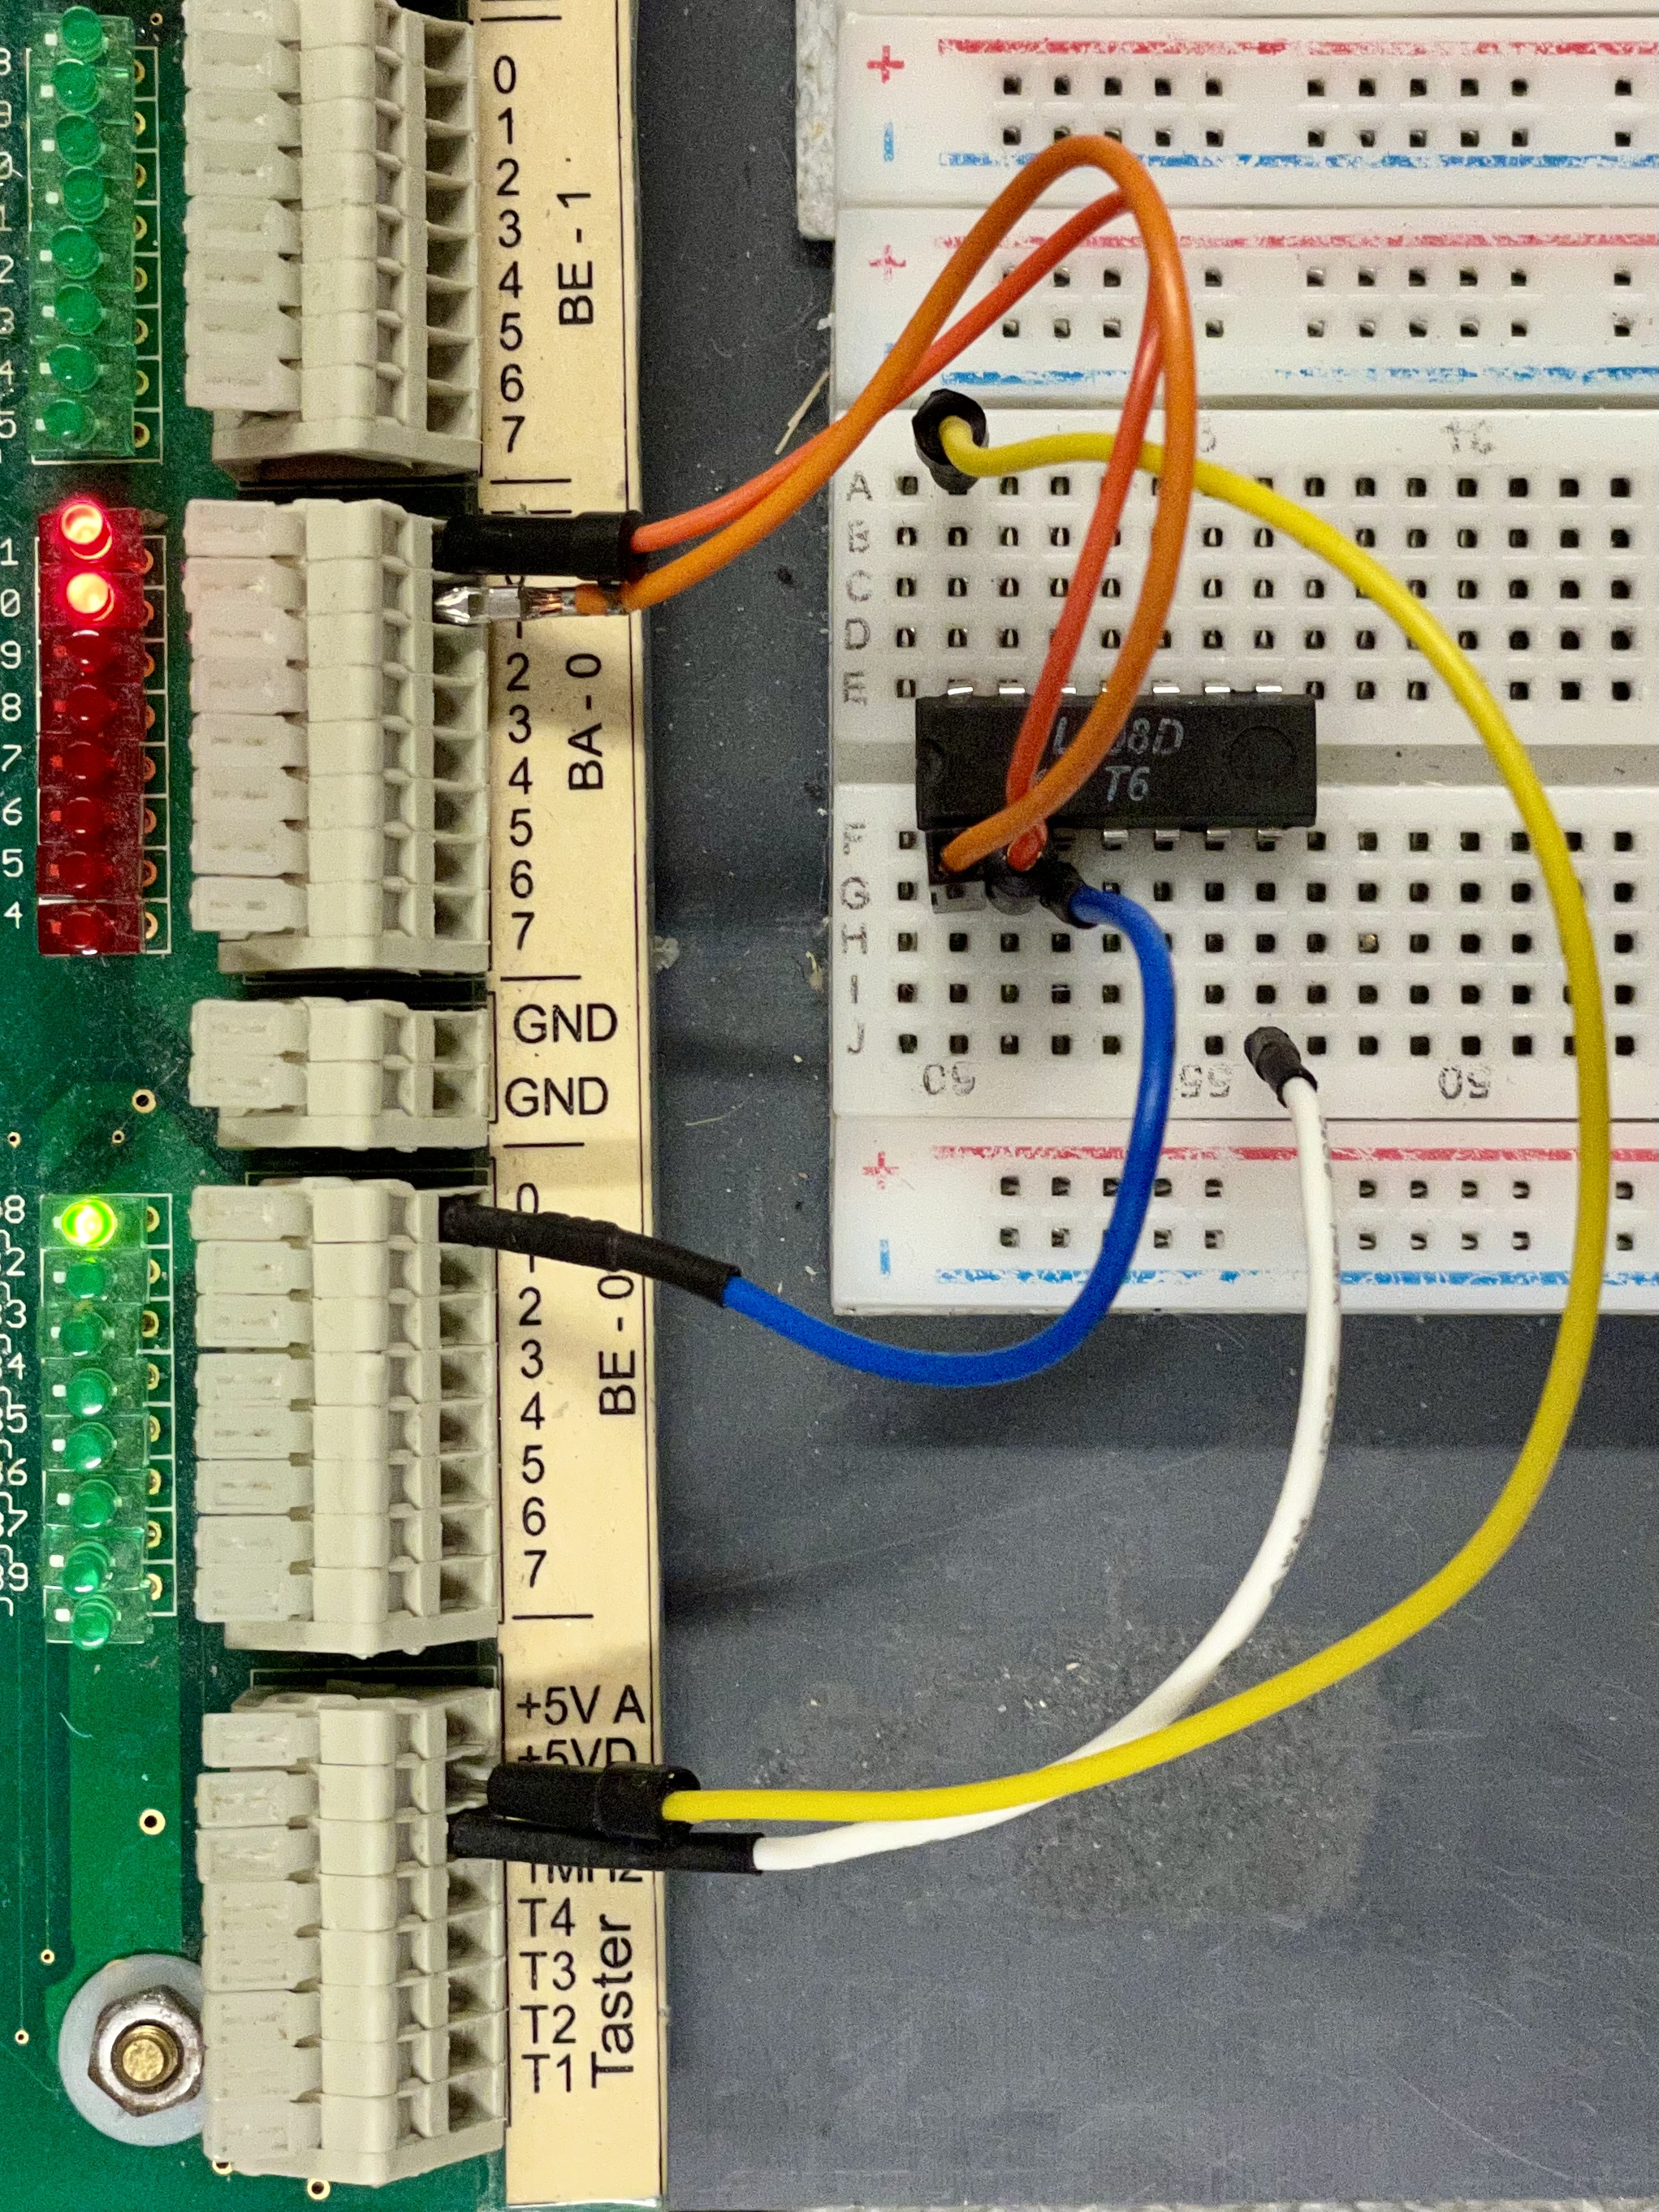
\includegraphics[width=.4\textwidth]{task11-1.JPG}
	\caption{Aufbau des verwendeten UND-Gatters}
	\label{task11-1}
\end{wrapfigure}

\paragraph{Aufgabenstellung}
Wählen Sie ein beliebiges Logikgatter, verbinden Sie dessen Eingänge mit dem B15-Board. Nutzen Sie das Monitor-Programm um die Wahrheitswertetabelle Ihres Logikgatters zu erstellen.

\paragraph{Vorüberlegung}
Ausgewählt wurde ein AND Gatter vom Typ \textit{DL008D}. Der Ausgang sollte erst durchgeschaltet werden, wenn beide Eingänge eingeschaltet sind.

\begin{wrapfigure}[2]{r}{.4\textwidth}
	\centering
	\begin{tabular}{|l|l|l|}
		\hline
		\textbf{$E_2$} & \textbf{$E_1$} & \textbf{$A$} \\ \hline\hline
		0          & 0          & 0          \\ \hline
		0          & 1          & 0          \\ \hline
		1          & 0          & 0          \\ \hline
		1          & 1          & 1          \\ \hline
	\end{tabular}
	\caption{Wahrheitswertetabelle der UND-Verknüpfung}
	\label{table:task11.1}
\end{wrapfigure}

\paragraph{Durchführung}
Das Gatter wird mit 5V Betriebsspannung über Pin 14 versorgt und über Pin 7 geerdet. Die Pins 1 und 2 sind Eingänge, dessen Ergebnis wird auf Pin 3 ausgegeben. Pin 1 wird mit Pin 0 und Pin 2 mit Pin 1 des Feldes BA-0 vom B15-Board verbunden. Die Ausgabe des Gatters wird auf BE-0 Pin 0 wiedergegeben. Der Aufbau kann Abbildung \vref{task11-1} entnommen werden. Zum testen dieser Schaltung wird der Wert von BA-0 mit den Binärkombinationen $00$, $01$, $10$ und $11$ nacheinander über das Monitor-Programm eingestellt. Die daraus entstandene Wahrheitswertetabelle ist in Abbildung \vref{table:task11.1} dargestellt.

\paragraph{Schlussfolgerung}
Das Ergebnis entspricht dem Erwartungswert. Der Versuch ist erfolgreich.

\newpage
\section{Aufgabe 11.2}

\paragraph{Aufgabenstellung}
Wählen Sie mindestens 3 beliebige Logikgatter aus. Erstellen Sie dar- aus eine Logikschaltung die mindestens 4 Eingangsvariablen hat. Entwickeln Sie mit Hilfe des B15 ein Programm welches automatisch die Wahrheitswertetabelle des Logikgatters ausgibt. Überprüfen Sie die Ausgabe.

\begin{wrapfigure}[22]{r}{.4\textwidth}
	\centering
	\begin{tabular}{|l|l|l|l|l|}
		\hline
		\textbf{$E_4$} & \textbf{$E_3$} & \textbf{$E_2$} & \textbf{$E_1$} & \textbf{$A$} \\ \hline\hline
		0             & 0             & 0             & 0             & 1          \\ \hline
		0             & 0             & 0             & 1             & 1          \\ \hline
		0             & 0             & 1             & 0             & 1          \\ \hline
		0             & 0             & 1             & 1             & 0          \\ \hline
		0             & 1             & 0             & 0             & 1          \\ \hline
		0             & 1             & 0             & 1             & 1          \\ \hline
		0             & 1             & 1             & 0             & 1          \\ \hline
		0             & 1             & 1             & 1             & 0          \\ \hline
		1             & 0             & 0             & 0             & 1          \\ \hline
		1             & 0             & 0             & 1             & 1          \\ \hline
		1             & 0             & 1             & 0             & 1          \\ \hline
		1             & 0             & 1             & 1             & 1          \\ \hline
		1             & 1             & 0             & 0             & 0          \\ \hline
		1             & 1             & 0             & 1             & 0          \\ \hline
		1             & 1             & 1             & 0             & 0          \\ \hline
		1             & 1             & 1             & 1             & 0          \\ \hline
	\end{tabular}
	\caption{Wahrheitswertetabelle der Schaltung}
	\label{table:task11.2}
\end{wrapfigure}

\paragraph{Vorüberlegung}
Zur verfügbaren Auswahl standen AND-, NAND-, NOR- und XOR-Gatter. XOR wurde schnell ausgeschlossen, da die gefundene Dokumentation zur Bedienung unzureichend für den Betrieb ist. Nach einigen Tests für eine Schaltung, die ein durchwachsenes und nicht einseitiges Ergebnis liefert, ergaben sich Probleme bei der Verwendung des NAND-Gatters. Eine passende Schaltung mit zwei AND- und einer NOR-Verknüpfung wurde gefunden. Das Programm, welches die Wahrheitswertetabelle ausgeben soll, sollte möglichst universell Einsetzbar sein. Daher sollte es eine variable Größe von Eingängen verarbeiten können. Da eine Eingabe von nötig ist, um dies umzusetzen, darf diese nur Zahlen im Bereich von 1 bis 255 akzeptieren. Das Ergebnis sollte gut lesbar in Tabellenform ausgegeben werden und Abbildung \vref{table:task11.2} entsprechen.

\paragraph{Durchführung}
Die Gatter AND \textit{(Typ DL008D)} und NOR \textit{(Typ DL002D)} werden auf dem Steckbrett wie in Abbildung \vref{task11-2} gezeigt positioniert und jeweils über die Pins 14 mit 5V Betriebsspannung versorgt und über Pin 7 geerdet. Der Pin 1 des AND-Gatter wird mit BA-0 Pin 0 und Pin 2 mit BA-0 Pin 1 des B15-Boards verbunden. Das Ergebnis beider Pins wird über Pin 3 mit Pin 3 des NOR-Gatters verbunden. Eine weitere UND-Verknüpfung wird mit Pin 13 über Pin 3 und Pin 12 des AND-Gatters über Pin 4 der Buchsen BA-0 des B15-Boards verbunden. Das Ergebnis dieser Verknüpfung wird von Pin 11 des AND-Gatters zu Pin 2 des NOR-Gatters geleitet. Die benötigten Eingänge zur Berechnung des NOR sind dadurch belegt und das Ergebnis dieser wird über Pin 1 des NOR-Gatters mit Pin 0 von BE-0 des B15-Boards verbunden. Die Schaltung ist nun Vollständig und kann ebenfalls Abbildung \vref{task11-2} entnommen werden. Folgende Formel beschreibt den Aufbau:
\[\neg{((a \land b) \lor (c \land d))}\]

\begin{figure}
	\centering
	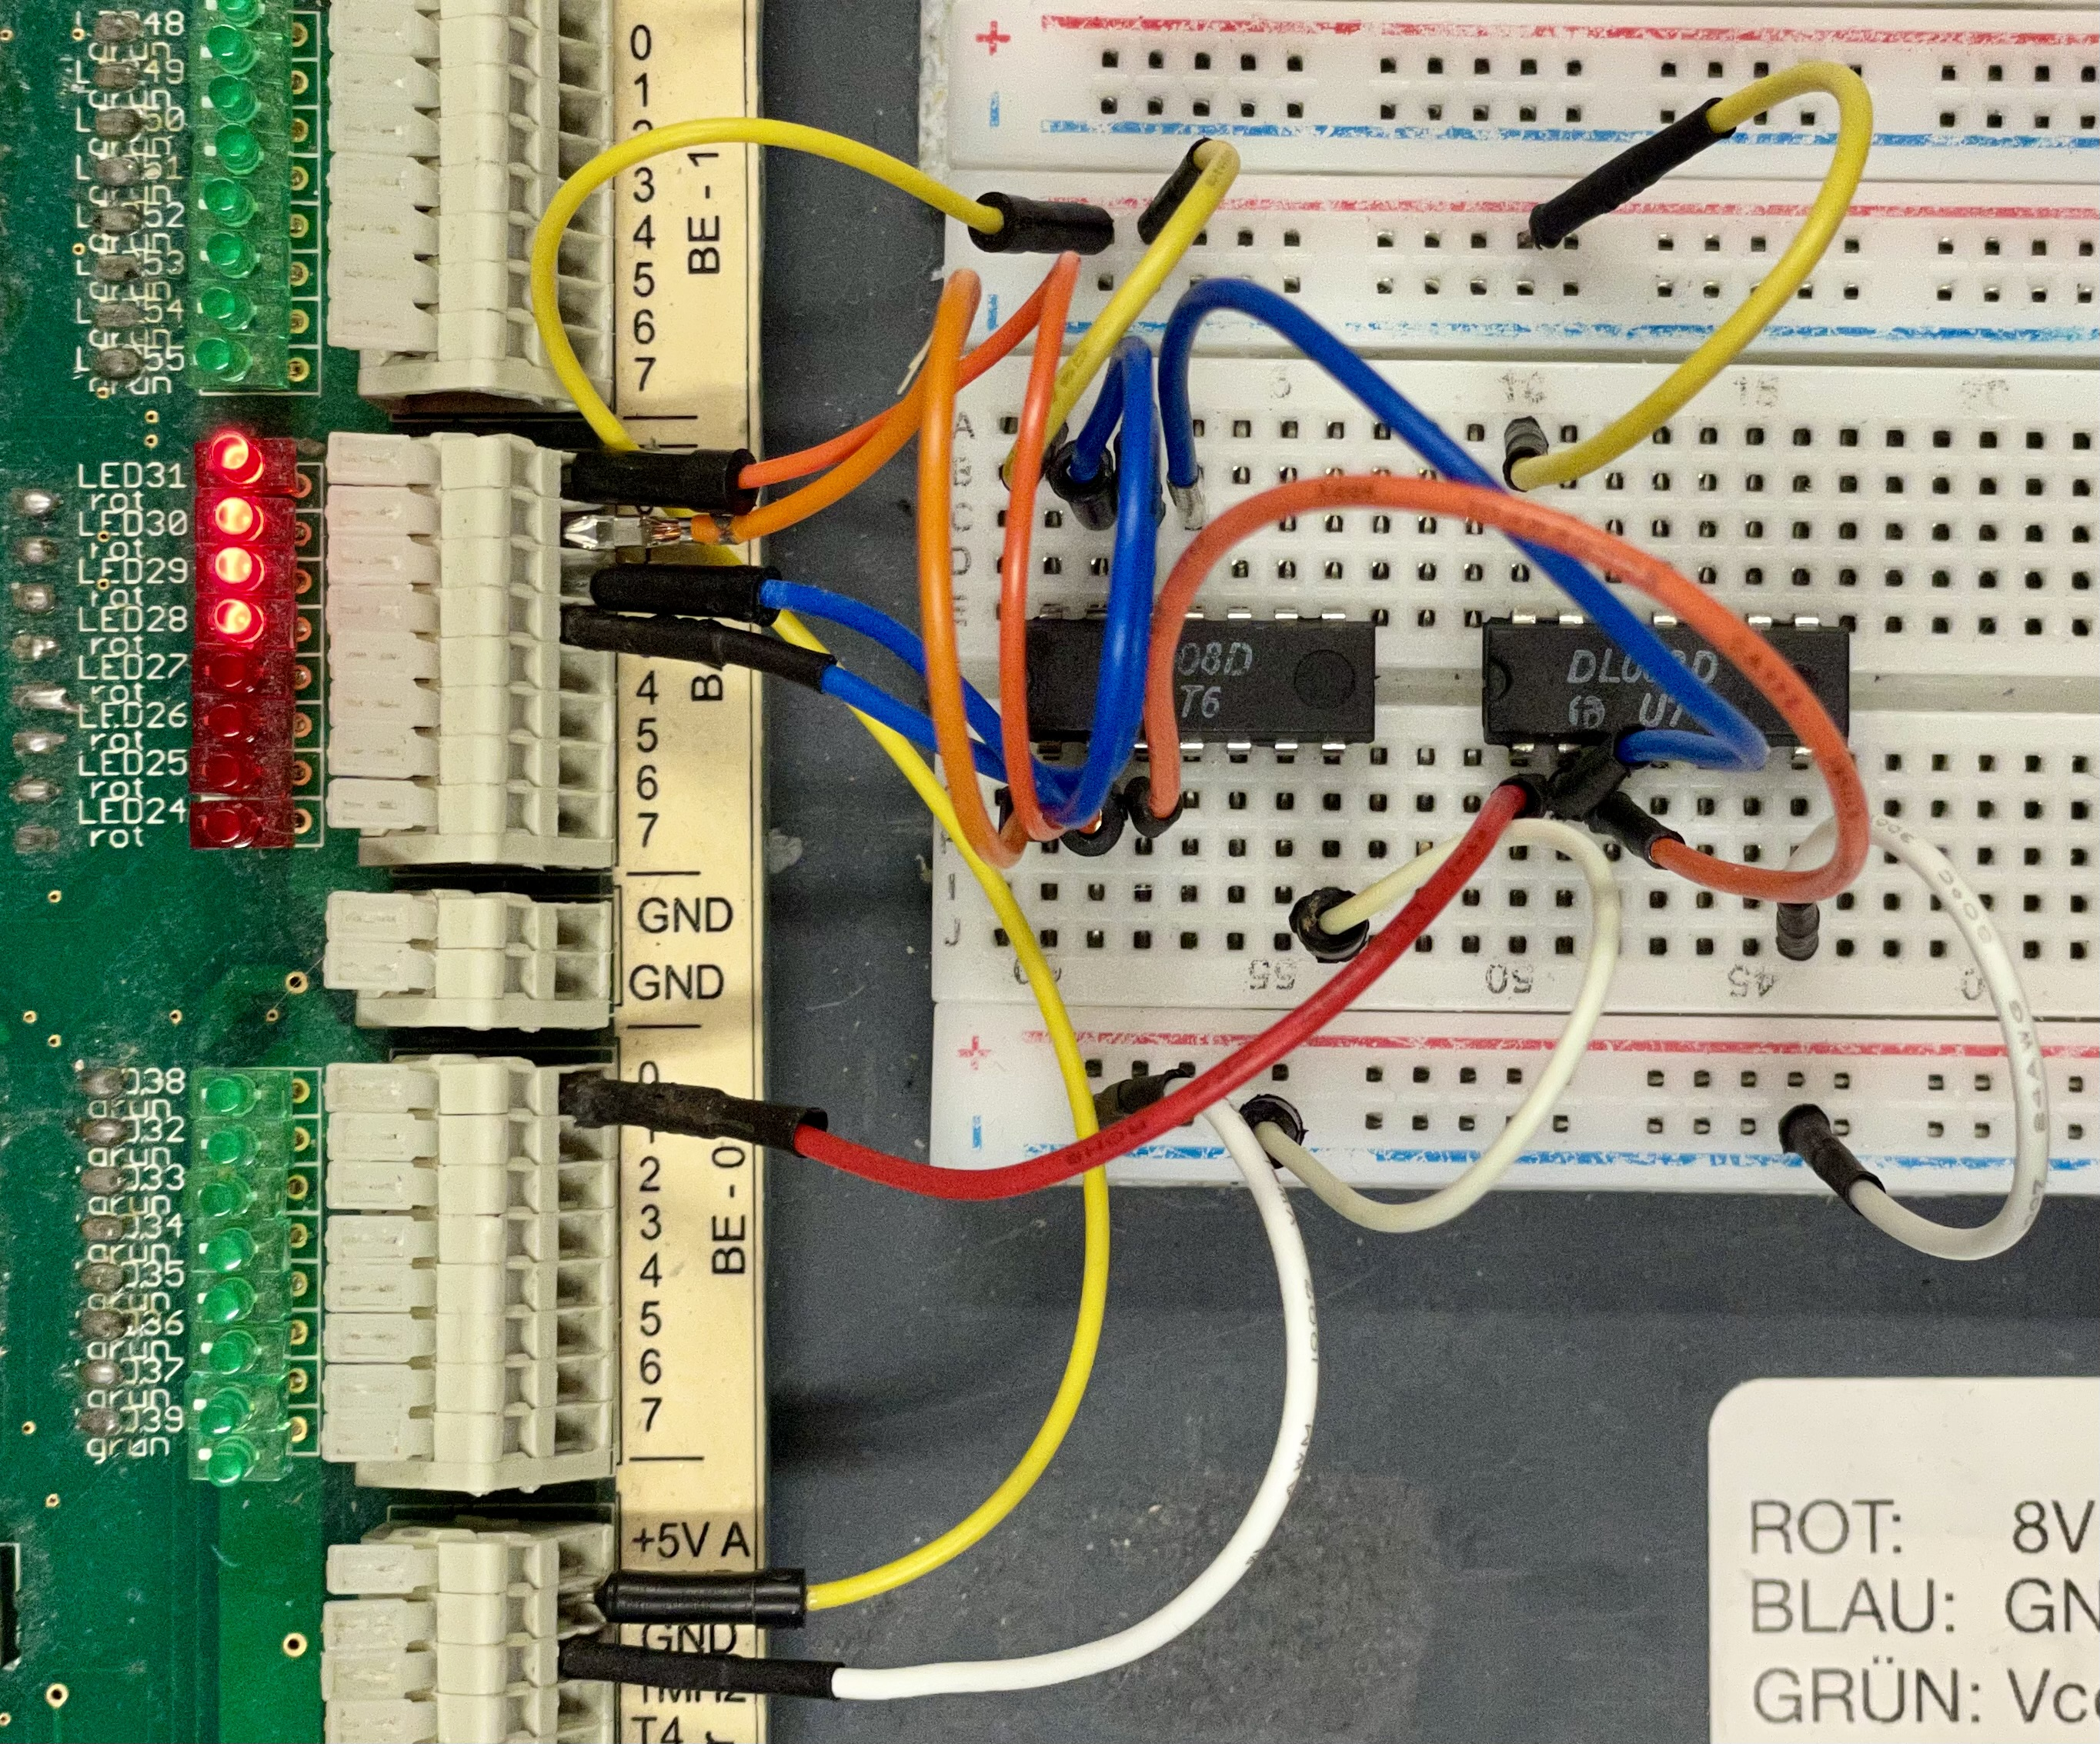
\includegraphics[width=.85\linewidth]{task11-2.JPG}
	\caption{Aufbau der Logischen Schaltung}
	\label{task11-2}
\end{figure}

\begin{figure}
	\centering
	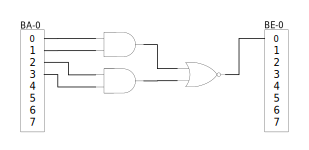
\includegraphics[width=.85\linewidth]{task11.JPG}
	\caption{Schaltplan}
	\label{task11-2-1}
\end{figure}

Das Programm baut eine Verbindung zum B15-Board auf, fragt den Benutzer nach der Testgröße und durchläuft alle Zahlen innerhalb dieser in aufsteigender Reihenfolge. Der Quelltext kann nachfolgend gelesen werden.

\fontsize{12pt}{12pt}\inputminted[linenos=true, breaklines]{cpp}{../task11/main.cpp}

\paragraph{Schlussfolgerung}
Das Ergebnis des Programms entspricht dem Erwartungswert. Der Versuch ist erfolgreich. Die exakte Ausgabe des Programms lautet:

\fontsize{10pt}{10pt}\inputminted[breaklines]{console}{../task11/output.txt}

\section{Aufgabe 11.3}
\paragraph{Aufgabenstellung}
Räumen Sie alle Kabel und Widerstände die Sie aus dem Widerstandssortiment von der Wand genommen haben wieder zurück.

\paragraph{Durchführung}
Das Netzteil wird ausgeschaltet und die Kabel zur Stromversorgung abgeklemmt. Die Widerstände werden in entsprechende Box zurückgelegt und die Kabel der Schaltungen einzeln vom Steckbrett gelöst und gesammelt in die Kabelbox gelegt. Mit dem Bauteilegreifer werden die verwendeten Logikgatter einzeln vom Steckbrett gelöst und in die entsprechende Sammelbox gelegt.

\paragraph{Schlussfolgerung}
Der Arbeitsplatz befindet sich in einem sauberen Zustand und kann wieder verwendet werden.